\documentclass[grad,lot,lof,11pt,oneside,onehalfspace]{RUthesis}
\usepackage{xspace,amsmath,amssymb}
\usepackage[squaren]{SIunits}
\usepackage{hyperref}

% Hyperref options for color/format of links
\hypersetup{
    colorlinks=true,  % false: boxed links; true: colored links
    linkcolor=black,   % color of internal links
    citecolor=black,   % color of links to bibliography
    filecolor=black,   % color of file links
    urlcolor=black     % color of external links
}


\newcommand{\be}{\begin{equation}}
\newcommand{\ee}{\end{equation}}
\newcommand{\ben}{\begin{equation*}}
\newcommand{\een}{\end{equation*}}
\newcommand{\bea}{\begin{eqnarray}}
\newcommand{\eea}{\end{eqnarray}}
\newcommand{\bean}{\begin{eqnarray*}}
\newcommand{\eean}{\end{eqnarray*}}
\newcommand{\dif}{\mathrm{d}}
\newcommand{\me}{\mathrm{e}}
\newcommand{\e}[1]{\ensuremath{\times10^{#1}}}

% Additional non-SI-units
% useful/specific to your field
\addunit{\dpi}{dpi}
\addunit{\tcid}{TCID\ensuremath{_{50}}}

\title{A proposed Defense Framework Against Adversarial Machine Learning Attacks Using Honeypots.}
\author{Fadi Younis}
\RUdegree{Master of Science}
\RUfield{Computer Science}
\RUsupervisor{Dr.\ Ali Miri}
\RUdepartment{Science}
\RUsubmitdate{September 14, 2012}
\RUaddress{Department of Science,\\
    Ryerson University,\\
    Toronto, Ontario \\
    Canada \\
    M5B 2K3}
\RUyear{2018}
\RUpastdegrees{B.Sc.\ Ryerson University, Toronto (ON), Canada, 2009}


\RUdedication{To my friends, My dear family and and wonderful colleagues, Without whom none of my success would be possible. }

% WARNING:
% MSc abstract should be at most 150 words not including title, name, etc.
% PhD abstract should be at most 350 words not including title, name, etc.
\RUabstract{
This is my wonderful abstract. I really like my abstract because it's so pretty. I've made sure it's less than 150 words if I'm a M.Sc.\ student and less than 350 words if I'm a Ph.D.\ student. I've not included any graphs, tables or references in it. If I really had to use symbols in my abstract I'd be sure to also explain right here what they stand for because I'm such a good student and I know all the thesis rules.
}

\RUacknowledgement{
Many people have contributed to my work here at Ryerson University. First I thank my supervisor Dr.\ Ali Miri for guiding my research, as well as providing many helpful suggestions throughout my time here. I would like to acknowledge the Department of Computer Science for providing me funding while I did my research. }

\begin{document}

\maketitle
 
\chapter{Introduction}
 In this chapter, we introduce the thesis problem setting in which Adversarial Examples occur and maliciously influence the prediction model (\textbf{Section 1.1}). Then, we provide an overview of the thesis problem subject matter (\textbf{Section 1.2}), the motivation for solving the problem follows after (\textbf{Section 1.3}). We then outline the goal(s) we hope to reach with our solution, by the end of this thesis (\textbf{Section 1.4}). Finally, we end the chapter with an outline for the remainder of this thesis (\textbf{Section 1.5}).
\section{Setting}
  Machine Learning, as we know it,  is exploding in development and demand, with utilization in critical applications, services and domains, not confined to one area of industry but several. With each day, more applications are harnessing the suitability of Machine Learning. To meet the ever increasing demand that this forefront is witnessing, tech giants such as Amazon, Google, Uber, Netflix, Microsoft and many others are providing their Machine Learning adjuncted products and services in the form of an online cloud service, otherwise known as\textit{ Machine-Learning-As-A-Service} (MLaaS)\cite{ribeiro_mlaas:_2015}. While the need for easily accessible Machine Learning tools is becoming readily available, the desire to personally customize and build these services from the ground up is actually decreasing and less relied upon. This is because users do not wish to spend countless hours training, testing and fine-tuning their machine learning models, they simply want to readily use them. While some users still prefer to ordain and control how their models are constructed and deployed, companies have undergone the effort to hide the internal complex mechanisms from most of their indolent users, and package them in non-transparent and easily customized services. Essentially, they provide their services in the form of a \textit{Black-Box}\cite{kurakin_adversarial_2016}\cite{papernot_practical_2016}. This opaque system container accepts some input and produces an output, but where the internal details of the model are hidden. However, like any application deployed, we cannot assume it is sited in a safe environment. There are security flaws and vulnerabilities in every man-made system and the container holding a MLaaS is no exception to the assumption. These weaknesses introduce a susceptibility to malicious attack(s), which is expected and almost always the case. Like any regular user, an adversarial attacker also does not have access to the internal
  components of the system, this knowledge might give a sense of security, and that the \textit{Black-Box} system is secure. But as we’ll see, this sense of security is only temporary, and only the beginning of the dangers to follow. 
\section{The Problem at a Glance}
  As we learned in the introduction of this chapter, Machine Learning Adversarial threats exist and are lurking close-by. The threat transpires when an attacker misleads and confuses the prediction model inside the cloud computing application offering the MLaaS, and allow malicious activities to go undetected \cite{papernot_practical_2016}. This  drives up the rate of false negatives, violating model integrity. These masqueraded inputs - called Adversarial Examples\cite{kurakin_adversarial_2016}, represent one of the recent threats to cloud services providing\textit{ Machine Learning as a Service} (MLaaS). These nonlinear inputs look familiar to the inputs normally accepted by a linearly designed classifier, but only appear that way. They’re maliciously crafted to exploit blind spots in the classifier boundary space, to mislead and confuse the learning mechanism in the classifier, to compromise the model integrity, post training. Most defenses aim at strengthening the classifier’s discriminator function, by training it on malicious input ahead of time to make it robust. Defense methods,  such as \textit{Regularization and Adversarial Training} have proven unsuccessful. The latter method, and others like it, alone, cannot be relied upon since they do not generalize well on new adversarial inputs.  This is evidently true in the case of a Black-Box (blind model) setting, where the adversary has access to only input and output labels, as mentioned. Our aim is to develop an adversarial defense framework to act as a secondary level of prevention to curb adversarial examples from corrupting the classifier, by deceiving the attacker.
\section{Motivation}
  Due to the exploding demand that machine learning is witnessing, the risk of adversarial threats has increased as well. For example, an attacker can maliciously fool an \textit{Artificial Neural Network} (ANN) classifier into allowing malicious activities to go undetected, without direct influence on the classifier itself (ref). These masqueraded inputs - called Adversarial Examples, represent one of the recent threats to cloud services providing Machine Learning as a Service (MLaaS). They’re maliciously crafted to exploit blind spots in the classifier boundary space, to mislead and confuse the learning mechanism in the classifier, post model training, to compromise the integrity of the model. As a result there has been an increased interest in defense techniques to combat them. \\
  Our challenge here lies in constructing an adversarial defense technique capable of deceiving the intrusive attacker and lure him away from the black-box target model. For purposes of our approach, we have decided to primarily use \textit{Adversarial Honey-Tokens}, which act as fictional digital breadcrumbs designed to lure the attacker and detectable using network sniffers used by the attacker. It is possible to generate a unique token for each item to deceive the attacker and track his abuse, however each token must be designed, generated and strategically embedded into the system to misinform and fool the adversary.\\
  previous research has aimed at strengthening the classifier’s discriminator function, by training it on malicious input to make it robust. Defense methods,  such as \textit{Regularization and Adversarial Training} have proven unsuccessful. The latter method has been criticized because it cannot be relied upon since they do not generalize well on new adversarial inputs \cite{rozsa_towards_2016}.  This is evidently true in the case of a Black-Box (blind model) setting, where the adversary has access to only input and output labels. We believe it is necessary to develop an adversarial defense framework to act as a secondary level of protection to prevent adversarial examples from corrupting the classifier, by deceiving the attacker. The majority of our is designing a distributed network of High-Interaction Honeypots as an open target for adversaries, these honeypot nodes act as sandboxes to contain the decoy neural network, collect valuable data and insight into adversarial attacks. We believe this might deter adversaries from attacking the target model. Other adversarial example defenses can also benefit and utilize this framework as an appendage in their techniques. Unlike other proposed defense models in literature, our model prevents the attacker from interacting directly with the target.\\
  We designed our defense framework to deceive the adversary in 3 steps, occurring sequential order of each other. The information collected from the attacker's interaction with decoy model could then potentially be used to  learn from the attacker, re-train and robustify the deep learning model in future training iterations. Our defense approach is motivated by trying to answer the following question \textit{"is there a possible way to fool the attacker and prevent him from learning behavior of the model"}. At its core, our intention is to devise a defense technique to both fool and prevent the attacker from interacting with the model.
\section{Thesis Goals}
Our thesis is as follows:\newline\\
\textit{"Given a deep learning model within a Black-Box setting and a intrusive attacker with an adversarial input capable of corrupting the model and misclassifying its labels there exists a defense framework to fool and deter the attacker's attempts. If building such a defense  framework is possible then there exists a way to prevent the attacker from learning the model's behavior and corrupting it."}\newline\\
The purpose of this work is to investigative the thesis above and build a an appropriate defense framework that implements it. Due to time and resource constraints, we limit our objectives to the following:
\begin{itemize}
	\item Propose an adversarial defense approach, that will act as a secondary level of defense to reinforce existing adversarial defenses. It aims to: 1) preventing the attacker from correctly learning the classifier labels, and approximating the correct architecture of the “Black-Box”, 2) luring the attacker away from the model towards a decoy model, and 3) create an infeasible computational work for the adversary, with no functional use.
	\item Evaluate performance of the proposed defense method in the thesis, its strengths, weaknesses, limitations and benefits. 
	\item Provide a detailed architecture and implementation of the \textit{Adversarial Honey-Tokens}, their design, features, usage, deployment and benefits.  
\end{itemize}
\section{Overview}
This thesis has  7 chapters. It is divided as follows:
\begin{itemize}
	\item\textbf{Chapter 1 -} gives a brief introduction to the problem at hand and its setting. This chapter also gives an overview of the thesis goals, and a breakdown of the outline.
	\item \textbf{Chapter 2 -} introduces the problem, and the motivation for solving it. It also introduces relevant concepts, such as \textit{Adversarial Machine Learning}, \textit{Transferability}, \textit{Deep Neural Networks}, \textit{Black-Box Systems}, and \textit{Honeypots}.
	\item \textbf{Chapter 3 -} gives a summary and critical evaluation of the related work(s) authored by other researchers on the topic of adversarial black box attacks and proposed defenses. 
	\item \textbf{Chapter 4 -} outlines the design and architecture of the defense approach. It also gives insight into the approach's setup, environment and limitations. It also shows how Honeypots can be used to curb adversarial attacks from influencing the model. 
	\item \textbf{Chapter 5 -} details the approach set-up, adversarial environment, limitations and evaluation criteria. 
	\item \textbf{Chapter 6 -} details implementation of the\textit{ Adversarial Honey-Tokens}, its features, usage, deployment and benefits. 
	\item\textbf{Chapter 7 -} summarizes the thesis, gives an overview of the contribution(s) made and suggests future research directions.
\end{itemize}


\chapter{Background}
The aim of this Chapter is to introduce the main problems and challenges involved in defenses against \textit{Adversarial Examples}. We also formulate important concepts so that they can be used to understand the upcoming chapters. We begin by throughly explaining concepts that will be important for the rest of this thesis. 
\section{Deep Learning and Security}
\subsection{Deep Learning}
\subsection{Vulnerabilities}
\subsection{Attacks on Deep Learning Networks}
\section{Adversarial Examples}
\subsection{Definition Adversarial Examples}
\subsection{Generation Adversarial Examples}
\subsection{Impact of Adversarial Examples}
\section{Adversarial Defenses}
\section{Transferability}
\newpage
\section{Black-Box Learning Systems}
\subsection{Black-Box Attack Models}
\subsection{Black-box Model Vs. Blind Model}
\subsection{Attack Approach}
\subsection{Vulnerability to Black-Box Attacks}

%==========================================================================
\newpage
\section{Honeypots}
The section focuses on Honeypots, we'll start with an in-depth definition of what a \textit{honeypot} is. Then, We dissect and explain the components comprising a honeypot and evaluate it's intrinsic value. This section also offers insight into how other security researchers have proposed using Honeypots for purposes of deception, as well as infrastructure security. 
\subsection{Concept of Honeypots}
A honeypot can be thought of as a fake system to collect intelligence on an adversary by inducing him to attack it. It's meant to appear and respond like a real system, in the production environment. However, the honeypot and the data inside is falsified and spurious. A honeypot has no real value. If it should become compromised, it poses no threat on the production environment\cite{lihet_how_2015}\cite{suo_research_2014}. Honeypots can be deployed with fabricated information that can be attractive to outside attackers, as well as re-direct attackers towards decoy systems and away from critical infrastructure \cite{guarnizo_siphon:_2017}.

\subsection{Classification of Honeypots}
Honeypots can be classified using several different criteria. However, for purposes of this thesis we classify them based on functionality and operation. 
\begin{itemize}
\item {\textbf{Research Honeypots} -}
They're Honeypots deployed with the highest level of risk associated with them, this is in order to expose the full range of attacks initiated by the adversary. They're mainly used to collect statistical data on adversarial activities inside the honeypot.\cite{lihet_how_2015}. They're more difficult to deploy, but this doesn't hinder from their use by organizations to study attacks and develop security countermeasures against them. Research Honeypots help understand the trends, strategies and motives behind adversarial attacks\cite{nawrocki_survey_2016}.
\item {\textbf{Production Honeypots} -}
They are Honeypots known for ease of deployment and utility, known for use in company production environment \cite{nawrocki_survey_2016}. Closely monitored and maintained, their purpose lies in their ability to be used in an organization's security infrastructure to deflect probes and security attacks. They're attractive as an option for ease of deployment and the sheer value of information collected on the adversary. 
\item {\textbf{Physical/Virtual Honeypots} -} 
Physical honeypots are locally deployed honeypots, being part of the physical infrastructure. considered to be intricate and difficult to properly implement \cite{lihet_how_2015}. On the other hand, virtual Honeypots are simulated systems (virtualized) by the host system to forward network traffic to the virtual honeypot \cite{nawrocki_survey_2016}.
\item {\textbf{Server/Client Honeypots} -} 
The main different between server and client honeypots is the former will wait until the adversary initiates the communication, while client Honeypots contact malicious entities and request an interaction \cite{nawrocki_survey_2016}. However, traditional Honeypots are usually server-based. 
\item {\textbf{Cloud Honeypots} -}
They are honeypots deployed on the cloud. This type of honeypot has many advantages, as well as restrictions. They are used by companies that at least have one part of their infrastructure on the cloud. Having the system (or part of it) in the cloud has its advantages, it makes it easy to install, update, as well as recover the honeypot in case of a corruption\cite{lihet_how_2015}.
\item {\textbf{Honey-tokens} -}
can be thought of as a \textit{digital} piece of information. It can manifested from a document, database entry, E-mail, or a credentials. In essence, it could be anything considered valuable enough to lure and bait the adversary. The benefit with these tokens is that they can be used to track stolen information and level of adversarial abuse in them system \cite{akiyama_honeycirculator:_2017} 
\end{itemize}
\subsection{Honeypot Deployment Modes}
Honeypots can be deployed in one of three deployment modes \cite{campbell_survey_2015}, they are:
\begin{itemize}
	\item \textbf{Deception} mode manipulates the adversary into thinking the responses are coming from the actual system itself. This system is used as a decoy and contains security weaknesses to attract attackers. According to researchers a honeypot is involved in deception activities if its responses can deceive an attacker into thinking that the response returned is from the real system. 
	\item \textbf{Intimidation} modes is when the adversary is aware of the measures in place to protect the system. A notification may inform the the attacker that the system is protect and all activity is monitored. This countermeasure may ward or scare off any adversarial \textit{novice}, and leave only the experienced adversaries with in-depth knowledge and competent skills to attack the system. 
	\item \textbf{Reconnaissance} mode is used to record and capture new attacks. This information is used to implement heuristics-based rules that can be applied in intrusion detection and prevention systems. With Reconnaissance,  the honeypot is used to detect both internal and external adversaries of the system. 
\end{itemize}
\subsection{Honeypot Role and Responsibilities}
The true value of Honeypots lay in their ability to address the issue of security in production system environments, they mainly focus ons:
\begin{itemize}
	\item \textbf{Interaction -}
	the honeypot should be responsible for interacting with the adversary. this pertains to acting as the main environment where the adversary becomes active and executes his attack strategy. 
	\item \textbf{Deception -}
	the honeypot should be responsible for deceiving the adversary. This pertains to the disguising itself as a normal production environment, when in fact it's a \textit{trap} or \textit{sandbox} designed to exploit the adversary. 
	\item \textbf{Data Collection -}
	the honeypot should be responsible for capturing and collecting data on the adversary. This information will potentially be useful for studying the attacker and his motivations. 
\end{itemize}
\subsubsection{Advantages of Honeypots}
Honeypots, alone, do not enhance the security of an infrastructure. However, we can think of them as subordinate to measures already in place. However, this level of importance does not take away from some distinct advantages when compared to other security mechanisms. Here, we highlight a few \cite{nawrocki_survey_2016}\cite:
\begin{itemize}
\item{\textbf{Valuable Data Collection} -}
Honeypots collect data which is not polluted  with noise  from production activities  and which is usually of high value. This makes data sets smaller and data analysis less complex.
\item{\textbf{Flexibility} -}
Honeypots are a very flexible concept to comprehend, as can be seen by the wide array of honeypot software available in the market. The indicates that a well-adjusted honeypot tool can be modified and used for different tasks, which further reduces architecture redundancy. 
\item{\textbf{Independent from Workload} -}
Honeypots do not need to process traffic directed or which originates from them. This means they are independent from the workload which the production system experiences. 
\item{\textbf{Zero-Day-Exploit Detection} -}
Honeypots capture any and every activity occurring within them, this could give indication to unseen adversarial strategies, trends and zero-day-exploits that can be identified from the session data collected.
\item{\textbf{Lower False Positives and Negatives} -}
any activity that occurs inside the server-honeypot is a considered to be out-of-place and therefore an anomaly, which is by definition an attack. Honeypots verify attacks by detecting system state changes and activities that occur within the honeypot container. This helps to reduce false positives and negatives.  
\end{itemize}
\subsubsection{Disadvantages of Honeypots}
Ultimately, no one security system or tool that exists is faultless. Honeypots suffers from some disadvantages,  some of them are \cite{nawrocki_survey_2016}:
\begin{itemize}
	\item{\textbf{Limited Field of View} -}
	a Honeypots is only useful if an adversary attacks them, and worthless if no one does.  if the honeypot is evaded by the adversary, and attacks the production system or target environment directly, it will not be detected.  
	\item{\textbf{Being Fingerprinted} -}  
	here, fingerprinting signifies the ability of the attacker to identify the presence of a honeypot. If the honeypot behaves differently than a real system, the attacker might identify and consequently detect it. If their presence is detected, the attacker can simply ignore the honeypot and attack the targeted  system instead. 
	\item{\textbf{Risk to the Environment} -}
	Honeypots might introduce a vulnerability to the production infrastructure environment, if exploited and compromised. And naturally, as the level of interaction (freedom) that the adversary has within the environment increases, so does the level of potential misuse and risk. The honeypot can be monitored, and the risk mitigated, but not completely eliminated.  
\end{itemize}

\subsection{Honeypots Level of Interaction}
A honeypot is considered to be an fake system, with no real value. It is built and designed to emulate the same tasks that a real production system can accomplish. However, these tasks are of no significance, hence compromising the honeypot poses no threat on the production environment .Honeypot system functionality can be categorized according to the level interaction the adversary has with the honeypot system environment \cite{lihet_how_2015}:
\begin{itemize}
	\item\textbf{Low-interaction Honeypot(LIHP) - }
	these type of system emulate only simple services like \textit{Secure Shell} (SSH), \textit{Hypertext Transfer Protocol}(HTTP) or \textit{File Transfer Protocol}(FTP). These systems are easily discoverable by attackers and provide the lowest possible level of security. However, they have a promising advantage, they are easy to install, configure and monitor. They should not be used in production environments, but for education and demonstration purposes. Some examples of such systems include \textit{Honeyperl}, \textit{Honeypoint}, and \textit{mysqlpot}.
	\item\textbf{Medium-interaction Honeypots(MIHP) -}
	this type of system is a hybrid, which lays in the middle ground between low/high interaction honeypots. This means that the honeypot is still an instance that runs within the operating system. However it blends in so seamlessly into the environment that it becomes difficult to detect by attackers lurking within the network. Some examples of such systems are \textit{Kippo} and \textit{Honeypy}.
	\item\textbf{High interaction Honeypot(HIHP) -}
	the main characteristic regarding High-Interaction Honeypots is that they're using a real live operating system. It uses more hardware resources and poses a major level risk on the rest of the production environment and infrastructure, when deployed. In order to minimize risk and prevent exploitation by an adversary, it is constantly under monitoring. Some examples of such systems are \textit{Pwnypot} and \textit{Capture-HPC}
\end{itemize}
\subsection{Honeypots in Deception}

\subsection{Conclusion}
As mentioned above, honeypots have a wide array of enterprise applications and uses. Currently, honeypot technology has been utilized in detecting \textit{Internet of Things} (IoT) cyberattack behavior, by analyzing incoming network traffic  traversing through IoT nodes, and gathering attack intelligence \cite{dowling_zigbee_2017}. In robotics, a honeypot was built to investigate remote network attacks on robotic systems\cite{irvene_honeybot:_2017}. Evidently, There is an increasing need to install \textit{red herring} system in place to thwart adversarial attacks before they occur and cause damage to production systems.   \\
One of the most popular type of honeypots technologies witnessing an increase in its popularity is High-Interaction-Honeypots (HIHP).  This type of honeypot is preferred since it provides a real-live system for the attacker to be active in. This property is valuable, since it captures the full spectrum of attacks launched by adversaries within the system. It us allows to learn as much as possible about the attacker, the strategy involved and tools used. Gaining this knowledge allows security experts to get insight into what future attacks might look like, and better understand the current ones. \\
High-Inter
where is the advantage here
whats the next chapter
\section{The Problem we Aim to Solve}

%===========================================================================

\chapter{Related Work}
In this Chapter we summarize and evaluate the work authored by other researchers on adversarial black box attacks defense techniques, as well as deception techniques and HoneyTokens.\\
The works below focus directly with the concept of defending adversarial examples by preprocessing of the data during the training phase of DNN model preparation. mention the challenge. That typically means influencing the effect the data will have on the underlying DNN model, and filtering our malicious perturbations inserted by an adversary that may corrupt it. Other works in this section focus on the role of cyber security defense through method of deception, specifically on the role of decoys and fake entities to deceive the attacker. Our challenge here is construct a secondary level of protection and defense, designed not to replace existing defense techniques ,but supplement and reinforce the mentioned defense frameworks below through means of adversary deception.\\
alternatives to current defense techniques include defense distillation 
The following papers and works deal directly with defenses against adversarial examples and other works associated with defense through deception using HoneyTokens:
\renewcommand{\theenumi}{\roman{enumi}}%
\begin{enumerate}
	\item \textit{Efficient Defenses Against Adversarial Attacks} this paper focuses on addressing the lack of efficient defenses against adversarial attacks undermining DNNs. This pressing need has been amplified by the fact that there isn't a unified understanding of how or why these adversarial attacks occur. The authors propose a solution which focuses on re-reinforcing the already existent DNN model and make it robust to adversarial attacks, attempting to fool it. The proposed solution focuses on utilizing two strategies to strengthen the model, the first strategy is using bounded RELU activation functions and second is augmented Gaussian data for training. The result of applying both strategies is a much smoother and stable model, without losing on the model's performance or accuracy.   
	\item \textit{Blocking Transferability of Adversarial Examples in Black-Box Learning Systems} - this paper \cite{hosseini_blocking_2017} is the closest academic paper, in terms of incentive and stimulus, for the purpose of developing our proposed auxiliary defense technique. An adversarial training approach is presented for robustifying Black-Box learning systems against Adversarial perturbations.  In this paper, the method of \textit{NULL labeling} is proposed, where adversarial examples are filtered out and discarded, instead of allowing them to be classified into respectful target label. The ingenuity of this approach lies how it is able to distinguish between clean and perturbed input. This method shows that it is capable of blocking adversarial transferability and resisting the adversarial input that exploit it. The latter is achieved  by mapping malicious input to a NULL label and allowing clean test data to be classified into its original label, all while maintaining prediction accuracy.
	\item \textit{Towards Robust Deep Neural Networks with BANG - } this paper \cite{rozsa_towards_2016} is another training approach for combating adversarial examples and robustifying the learning model. The authors propose this technique in response to the abnormal and mysterious nature of adversarial examples and the reason for their existence in Deep Neural Networks (DNNs). For this very purpose, the authors present a data training approach, known as \textit{Batch Adjusted Network Gradients} or \textit{BANG}. This method works by attempting to balance the causality that each input element has on the node weight updates. This achieves enhanced stability in the model by forming \textit{flatter} areas in the classification region and it becomes robust to input distortions that work on exploiting this. This method is designed to avoid instability brought about by the adversarial examples. The latter method achieves good results without manipulating the training data and low computational cost, while maintaining classification accuracy. 
	\item \textit{HoneyCirculator: distributing credential HoneyToken for introspection of web-based attack cycle} -  in this paper \cite{akiyama_honeycirculator:_2017}
	\item \textit{A Survey on Fake Entities as a Method to Detect and Monitor Malicious Activity - } this survey paper \cite{rauti_survey_2017} serves as an examination the concept of \textit{fake entities}, which my thesis defense relies heavily on. What makes fake entities so attractive as an asset, to the authors, is how inexpensive, lightweight and easy-to deploy they are, compared to other security mechanisms. Simply put, they're digital objects intended to be accessed by the attacker. Once in possession by an attacker, the defender is notified and can begin monitoring the attacker's activity. the main concern for the authors is designing convincing fake data to deceive to attract and fool an adversary. Generally, the defender should design fake entities which are \textit{attractive} to the attacker, while not revealing important or compromising information to the attacker, and learn as much as possible about the attacker. As the threat of adversarial attacks increases, so will the need for novelty in the approach to combat it.
	\item \textit{Designing Adaptive Deception Strategies - } this paper \cite{faveri_designing_2016} was used to derive the initial motivation for using Honeypots as an ad-hoc method approach to curb adversarial attacks in this thesis. Here, the authors strongly advocate for the use of deception-based strategies in defense architectures to mislead and confuse attackers. Specifically, the authors suggest compounding deception techniques into the traditional software life-cycle approach, to be used when designing adaptive systems designed to thwart adversaries, based on the attacker's goals, monitoring channels, metrics, and risks. The utility of this approach is shown through the use of a detailed use-case where a deception strategy is used build a smartphone application that synchronizes erroneous data with a database to deceive the attacker. 
    \item \textit{Deception Planning Models for Cyber Security - in this paper} the authors focus on the role that deception plays has when it comes to defense in Cyber Security. Here, the authors identify 20 important features that aid in characterizing and integrating deception as a method of defense in design of deception-based frameworks. For instance, what is the scope of deception when it comes to design, which tools are being used to deceive the adversary, how is deception integrated into other parts of the defense framework. Other features include, deception metrics, risks, bias exploitation, deploy and execution, timing and termination plan. This survey outlines important factors that should considered when integrating deception into any defense framework. \\
	There is also extensive work done on utilizing adversarial transferability in other forms of adversarial attacks, deep learning vulnerabilities in DNNs, and black-box attacks in machine Learning. Other interesting works include utilizing honeypots in defense techniques, such as design and implementation of a honey-trap \cite{egupov_development_2017}, deception in distributed system environments \cite{soule_enabling_2016}, and using containers in deceptive honeypots \cite{kedrowitsch_first_2017}.
\end{enumerate}


\chapter{Proposed Defense Approach}
\label{chap-math}
\section{Motivation}
\section{Approach}
\section{Attacker}
\subsection{Attack Setting}
\subsection{Attack Goal}
\subsection{Attacker Knowledge}
\subsection{Attacker Capabilities}
\section{Adversarial Honeypot Network Overview}
\section{Individual Honeypot Topology}
\section{Threat Model}
\section{Target and Decoy Model}
\section{Target Model}
\subsection{Purpose}
\subsection{Architecture and Topology}
\subsection{Training, Testing and Validation}
\newpage
\section{Attracting The Adversary}
\subsection{Adversarial Tokens}
\subsection{Weak TCP/IP ports}
\subsection{Decoy Target Model}
\section{Detecting Malicious Behavior}
\section{Monitoring the Adversary}
\section{Launching The Attack}
\section{Defending Against Attack}
\section{Deployment}
\section{Scalability}
\section{Security}




\section{Mathematical models of virus dynamics}

The basic model of virus dynamics can be written as follows \cite{nowak-may, perelson02, bonhoeffer97}: 

\begin{align*}
\frac{\dif T}{\dif t} &= -\beta T V \\
\frac{\dif I}{\dif t} &= \beta T V - \delta I \label{basic}\\
\frac{\dif V}{\dif t} &=  p I - c V\ .\nonumber
\end{align*}
where $T$ is something something.


\section{Shape of the viral titer curve}

The virus spread and kills everything. This is well illustrated in Figure \ref{kinetics} where the kinetics of the infection are shown for three different viral production rates of the secondary cell population for the case where these cells are 1,000-fold harder to infect than cells of the default type. 
\begin{figure*}
\begin{center}
\resizebox{0.31\textwidth}{!}{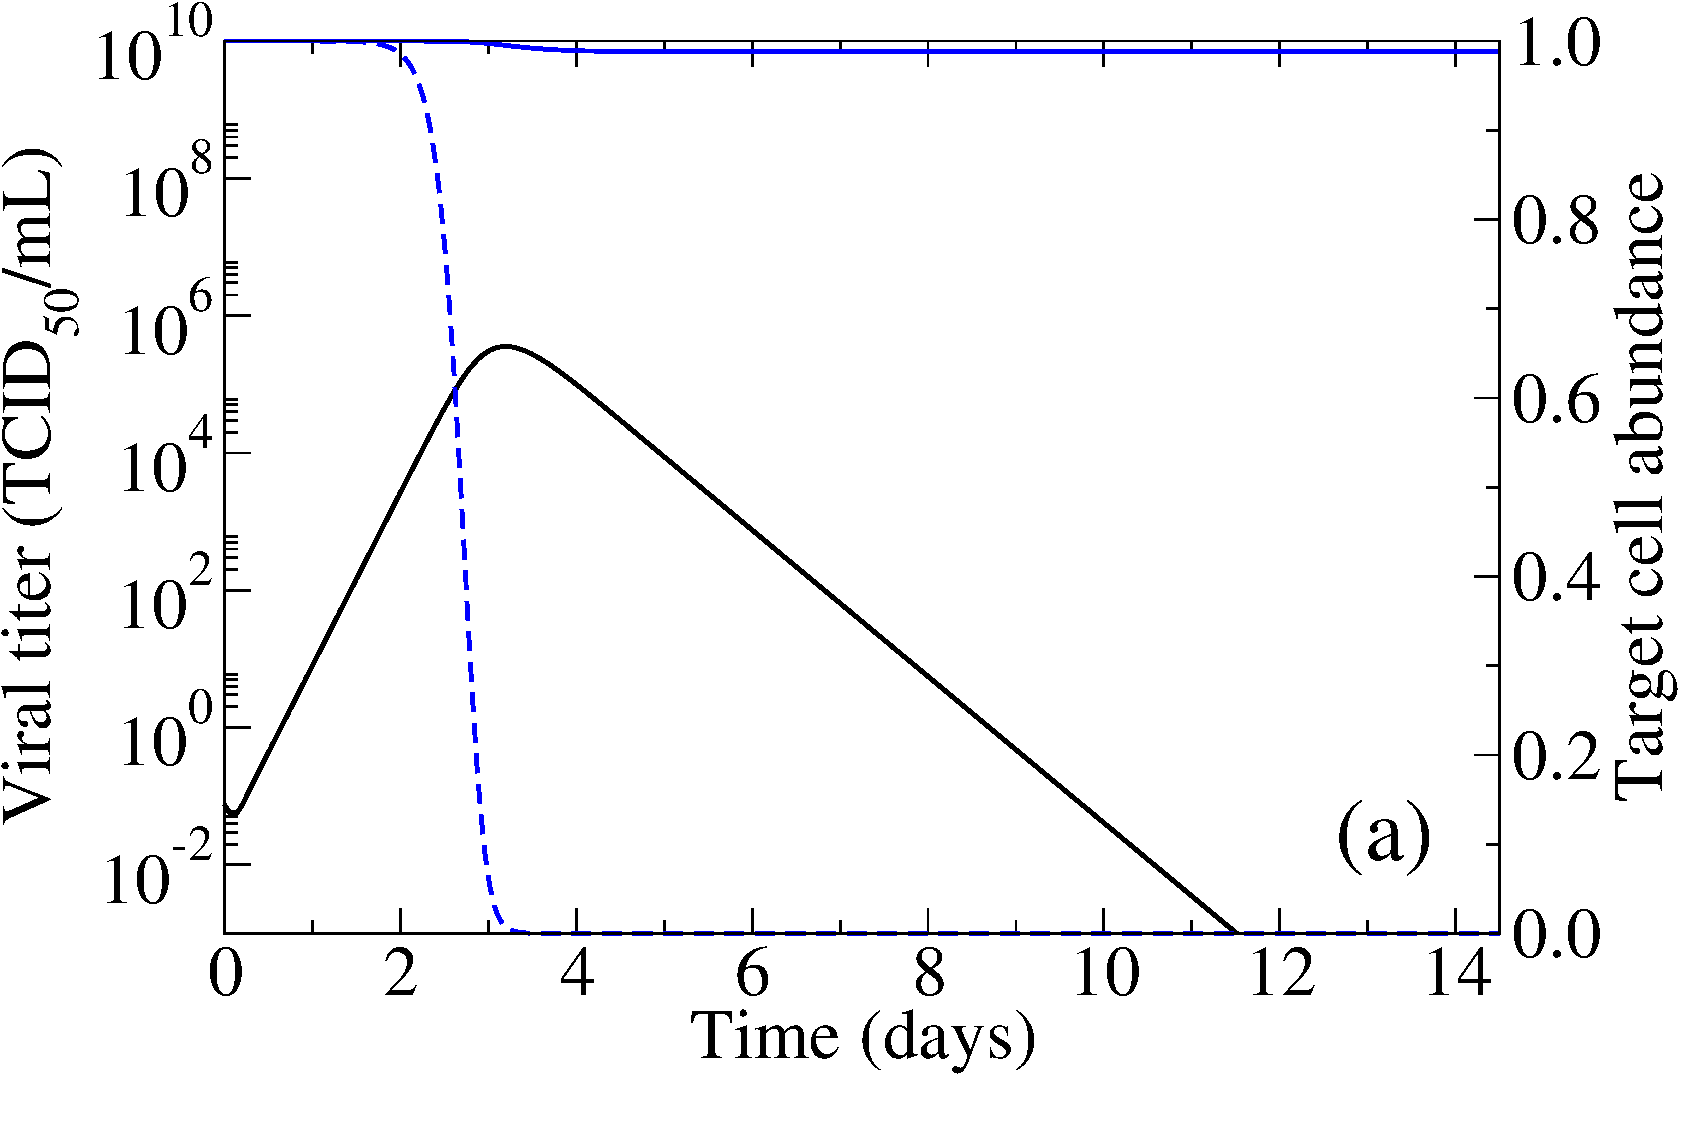
\includegraphics{myfig}}
\resizebox{0.31\textwidth}{!}{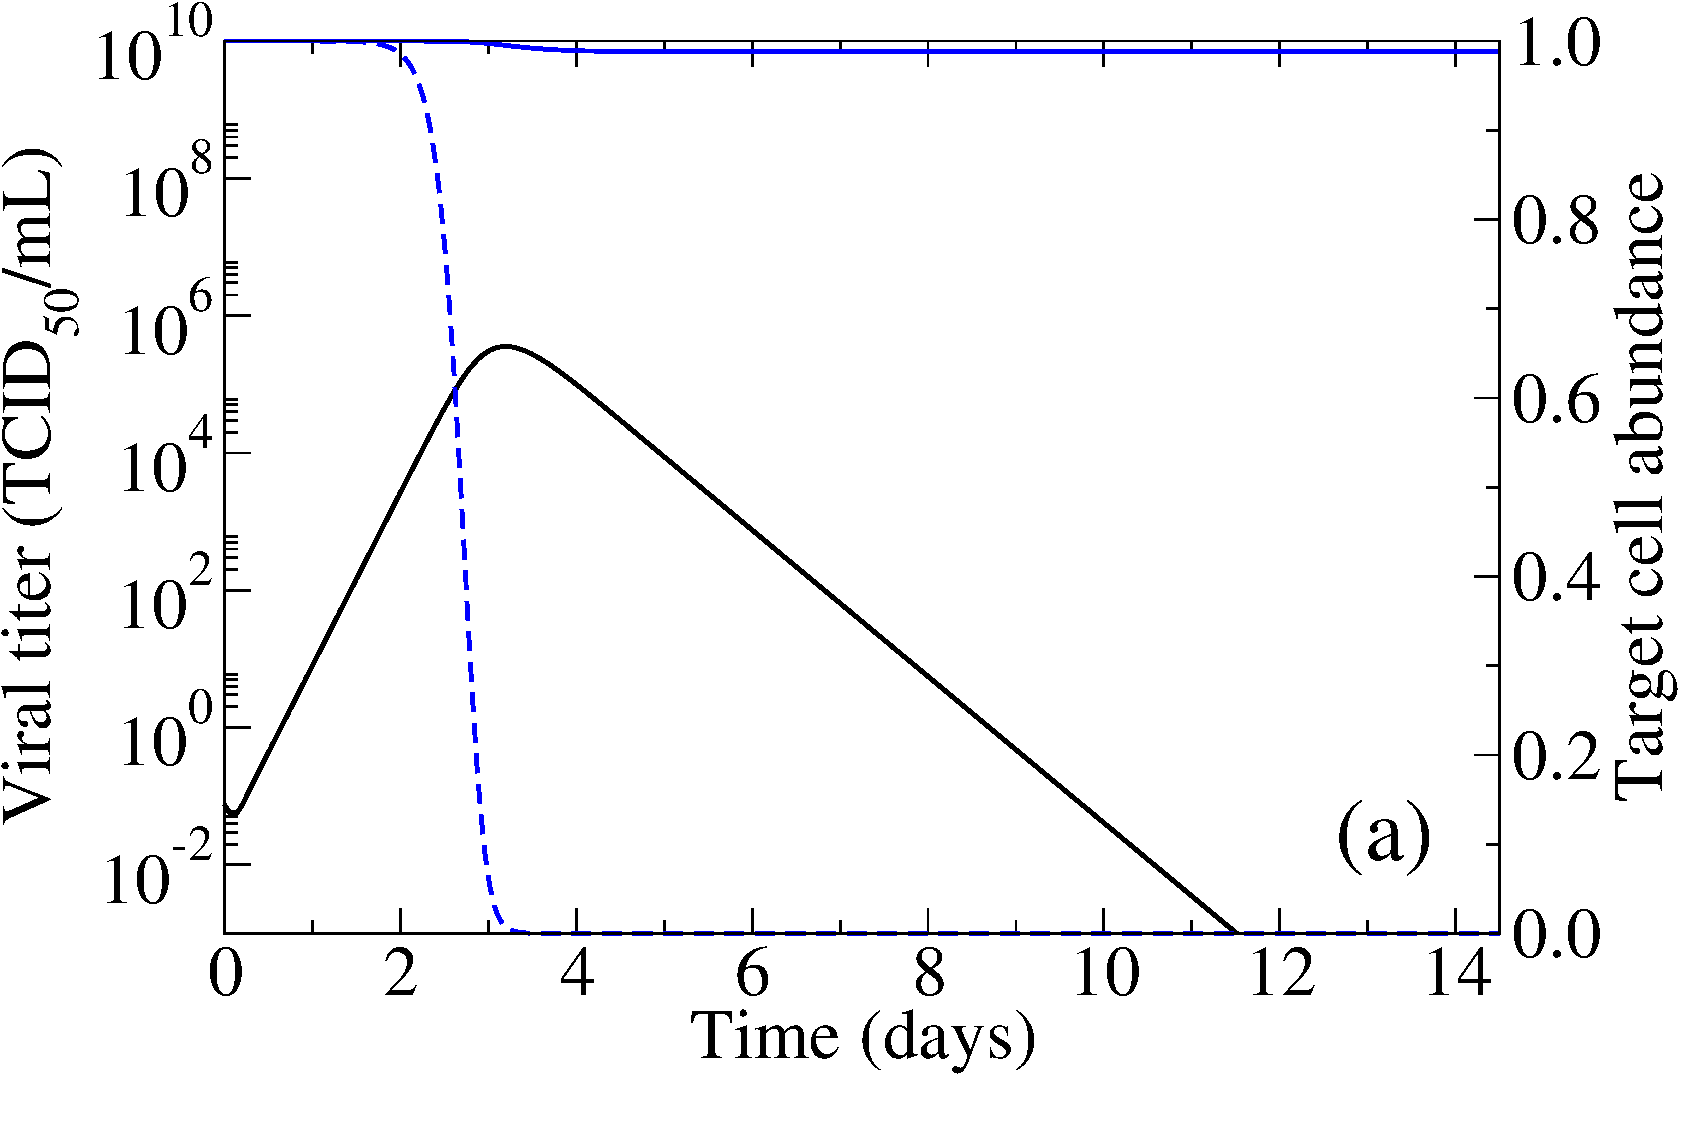
\includegraphics{myfig}}
\resizebox{0.31\textwidth}{!}{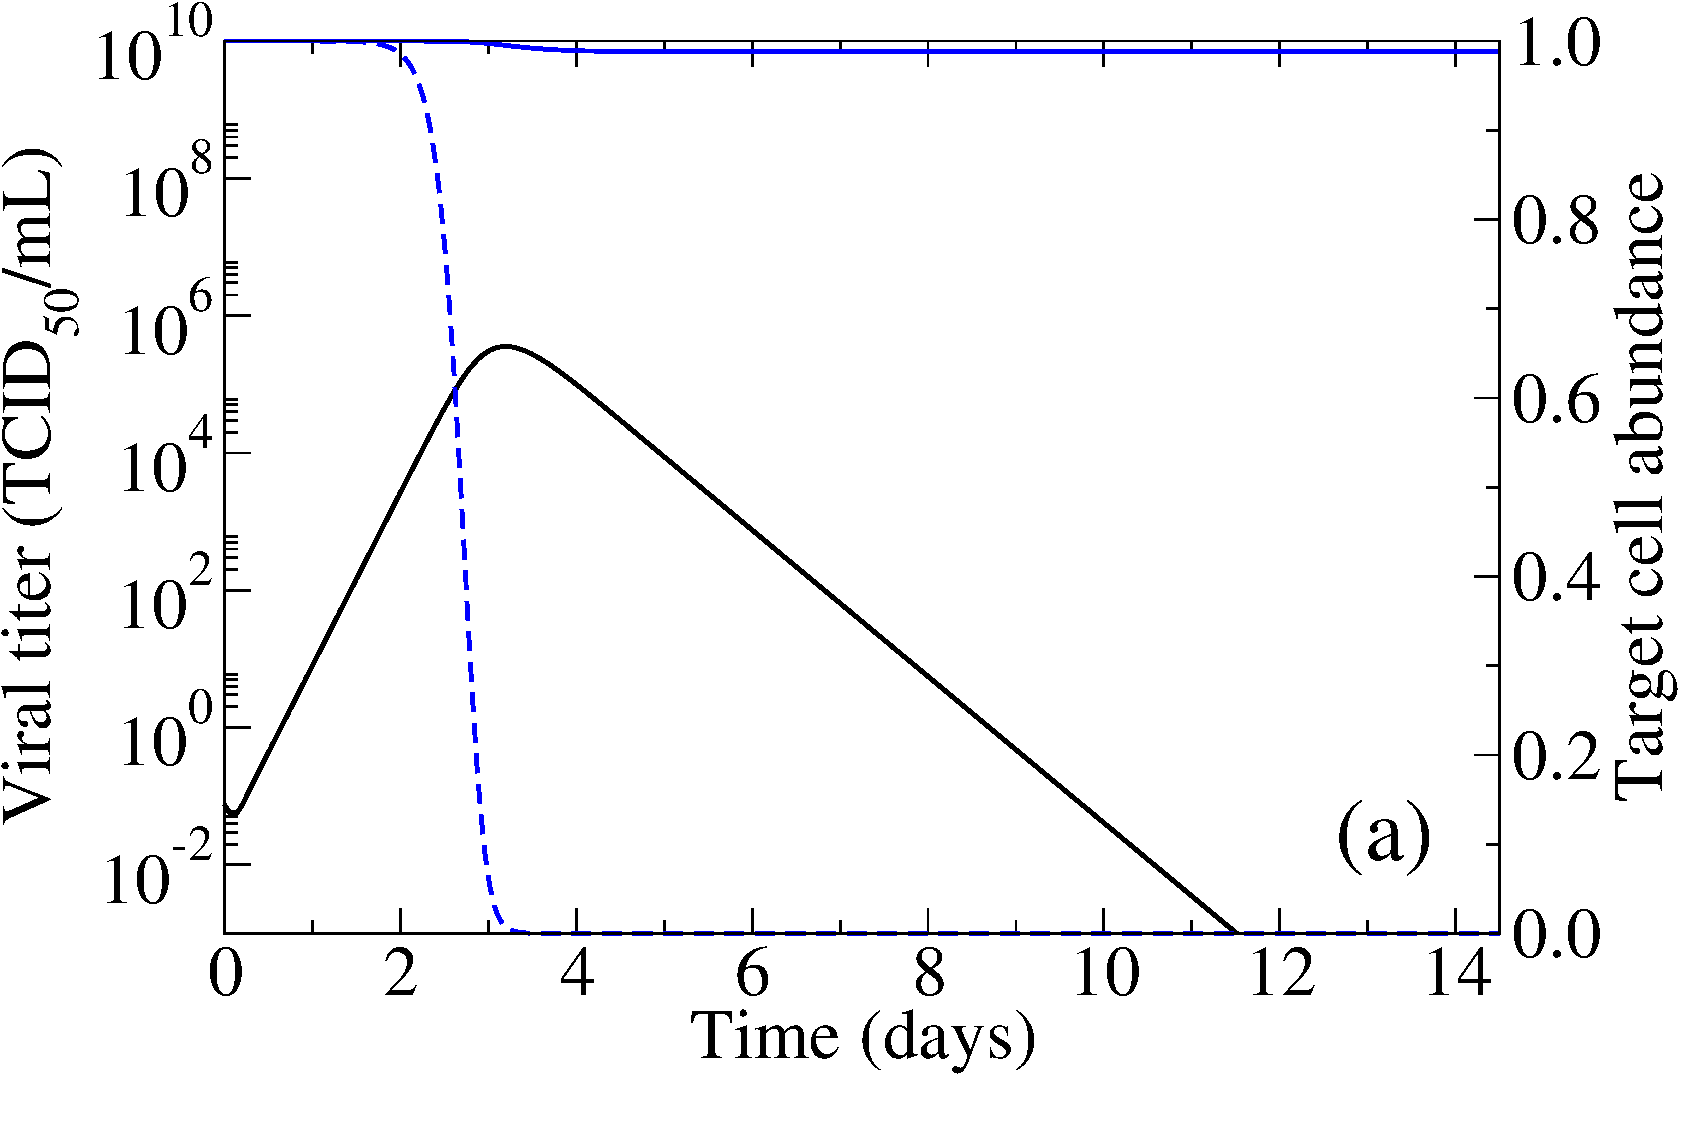
\includegraphics{myfig}}
\end{center}
\caption[Example figure file]{\textbf{An example illustrating how to include figure files.} I can not only display figures, but I can resize them so they look just right to appear side-by-side. This is how you produce multiple-panel images as a single figure. In addition, if your figure file is generated from some sort of model, you can refer to the table where the data or model parameters are listed. For example, you could say: All parameters are as in Table \ref{params}.}
\label{kinetics}
\end{figure*}
When secondary cells produce only 10-fold more virus than cells of the default type, the infection is mostly limited to the default cell population as the amount of virus produced is not sufficient for the infection to spread to the secondary cell population. Increasing the production rate to 100-fold more than cells of the default type results in a sufficient amount of virus being produced to sustain a slow growing infection within the secondary cell population, leading to long-lasting, high-levels of viral titer. Finally, increasing the viral production rate to 1,000-fold more than the default cell type allows the infection to successfully infect and decimate both cell populations rapidly. From these results, we see that there appears to be a relationship between the secondary cells' susceptibility to infection and their viral production rate which leads to a severe and sustained infection.

Note that all parameters use to produce our simulations can be found in Table \ref{params}.


\chapter{Evaluation and Discussion}
\chapter{Implementation and Discussion}
\section{Background}
\section{Architecture}
\section{Features}
\section{Functionality}
\section{Usage}
\section{Deployment}
\section{Integration}
\section{Benefits}
\section{Future Work}
\appendix % Optional: only if you need one

\chapter{Summary and Contributions}
\section{Summary}
\section{Discussion}
\section{Contributions}
\section{Future Work}
\section{Conclusion}

\chapter{Appendix A}

\chapter{Appendix B}


blah blah

\subsection{An appendix subsection if required}

blah blah blah.

\chapter{The second appendix chapter}

\section{A section in my second appendix chapter}

blah blah.

\subsection{Just making sure it all works}

blah blah blah.

% This typesets your bibliography
% based on the grad-thesis.bib file
\cleardoublepage
\bibliographystyle{abbrv}
\addcontentsline{toc}{chapter}{Bibliography}
\bibliography{Thesis}%UPDATE THIS!!!!!!!!!!!!!!


\end{document}
